\documentclass[12pt]{article}
\usepackage[utf8]{inputenc}
\usepackage[T1]{fontenc}
\usepackage{graphicx}
\usepackage{subcaption}
\usepackage{amsmath}
\usepackage{fancyhdr}
\usepackage{geometry}
\usepackage[english]{babel}
\usepackage{csquotes}
\usepackage{hyperref}
\usepackage{url}
\usepackage{listings}
\usepackage{float}
\usepackage{booktabs}
\usepackage{array}
\usepackage{tikz}
\usetikzlibrary{
    shapes.geometric, shapes.misc,
    arrows.meta, positioning, fit,
    backgrounds, calc, decorations.pathreplacing,
    automata
}
\usepackage{setspace}

\lstset{
    language=C,
    basicstyle=\ttfamily\small,
    numberstyle=\tiny,
    frame=single,
    breaklines=true,
}

% ── TikZ styles ────────────────────────────────────────────────────────────────
\tikzset{
  comp/.style={rectangle, draw, rounded corners=3pt,
               minimum width=2.8cm, minimum height=0.75cm,
               align=center, font=\small},
  hw/.style={comp, fill=gray!20},
  driver/.style={comp, fill=blue!15},
  service/.style={comp, fill=green!15},
  task/.style={comp, fill=orange!20},
  app/.style={comp, fill=yellow!20},
  arr/.style={-Stealth, thick},
  biarr/.style={Stealth-Stealth, thick},
  layer/.style={rectangle, draw, minimum height=0.9cm,
                align=center, font=\small\bfseries},
  cls/.style={rectangle, draw, font=\small, text width=2.8cm,
              minimum width=3.0cm, inner sep=3pt},
  hdr/.style={cls, fill=gray!10, align=center, font=\small\bfseries},
  uses/.style={-Stealth, dashed, thick},
  impl/.style={-Stealth, thick},
  state/.style={circle, draw, fill=blue!10, minimum size=2.0cm,
                align=center, font=\small\bfseries},
}
% ───────────────────────────────────────────────────────────────────────────────

\linespread{1.25}
\setlength{\parindent}{0.8cm}
\setlength{\parskip}{0em}
\renewcommand{\headrulewidth}{0pt}
\geometry{a4paper, portrait, margin=1in}
\setlength{\headheight}{14.49998pt}

\begin{document}
\begin{titlepage}
   \begin{center}
    \textsc{\large Ministry of Education of Republic of Moldova}\\[0.5cm]
    \textsc{\large Technical University of Moldova}\\[0.5cm]
    \textsc{\large Faculty of Computers, Informatics and Microelectronics}\\[0.5cm]
    \textsc{\large Software Engineering Department}\\[1.2cm]

    \vspace{25mm}

    {\LARGE \textbf{\textsc{Embedded Systems}}}\\[0.5cm]
    \textsc{\large Laboratory No. 1.5}\\[0.5cm]

    \newcommand{\HRule}{\rule{\linewidth}{0.5mm}}
    \vspace{80mm}

    \begin{minipage}[t]{0.4\textwidth}
    \begin{flushleft} \large
    \emph{Author:} \\
    Vladimir \textsc{Vitcovschii}\\
    std. gr. FAF-231
    \end{flushleft}
    \end{minipage}
    ~
    \begin{minipage}[t]{0.4\textwidth}
    \begin{flushright} \large
    \end{flushright}
    \end{minipage}\\[3cm]

    \vspace{5mm}
    \large Chi\c{s}in\u{a}u 2026\\[0.5cm]

    \vfill
    \end{center}
\end{titlepage}

\clearpage
\tableofcontents
\clearpage

\setcounter{page}{2}
\pagestyle{fancy}
\fancyhf{}
\rhead{\thepage}
\lhead{FAF-231 Vitcovschii Vladimir; Laboratory Work No. 1.5}

% ─────────────────────────────────────────────────────────────────────────────
\section{The Purpose of the Work}
% ─────────────────────────────────────────────────────────────────────────────

The purpose of this laboratory work is to develop a binary signal monitoring application using FreeRTOS on an ATmega2560 microcontroller. The application reads an analog NTC thermistor sensor, converts the ADC value to temperature using the Steinhart--Hart equation, and applies threshold alerting with hysteresis and debouncing. The focus is on correct signal acquisition, binary threshold classification with noise-resistant state transitions, and real-time display of sensor status via serial STDIO.

% ─────────────────────────────────────────────────────────────────────────────
\section{Objectives of the Work}
% ─────────────────────────────────────────────────────────────────────────────

The task requires implementing a temperature monitoring system on an ATmega2560 with FreeRTOS, using three concurrent tasks:
\begin{itemize}
  \item \textbf{Task~1 --- Sensor Reader}: Read the NTC thermistor via ADC every 50\,ms, convert the raw value to temperature in tenths of \(^{\circ}\)C using the Steinhart--Hart equation, and store the result in shared memory under mutex protection.
  \item \textbf{Task~2 --- Threshold Alert}: Every 50\,ms, compare the current temperature against a hysteresis band (alert activates above 30\,\(^{\circ}\)C, deactivates below 28\,\(^{\circ}\)C). Apply a debounce counter (5~consecutive samples) to confirm state changes. Control green (normal) and red (alert) LEDs.
  \item \textbf{Task~3 --- Display}: Every 500\,ms, snapshot the shared data under mutex and emit a formatted status line via \texttt{printf\_P} showing raw ADC, temperature, threshold state, debounce counter, and alert status.
  \item Use a single mutex (\texttt{xLab5Mutex}) to protect all shared volatile data from concurrent access.
  \item Implement the NTC sensor driver with Steinhart--Hart temperature conversion.
  \item All configuration values (pins, thresholds, timing) must be named constants --- no magic numbers.
\end{itemize}

% ─────────────────────────────────────────────────────────────────────────────
\section{Domain Analysis}
% ─────────────────────────────────────────────────────────────────────────────

\subsection{NTC Thermistor and Voltage Divider}

A Negative Temperature Coefficient (NTC) thermistor is a resistor whose resistance decreases as temperature increases. The thermistor used in this application has a nominal resistance of 10\,k\(\Omega\) at 25\,\(^{\circ}\)C and a Beta constant (\(B\)) of 3950.

The thermistor is connected in a voltage divider with a fixed 10\,k\(\Omega\) resistor:
\begin{equation}
V_{ADC} = V_{CC} \cdot \frac{R_{NTC}}{R_{fixed} + R_{NTC}}
\label{eq:vdiv}
\end{equation}

The ATmega2560's 10-bit ADC converts this voltage to a digital value in the range [0, 1023]. The NTC resistance can be recovered from the ADC reading:
\begin{equation}
R_{NTC} = R_{fixed} \cdot \frac{ADC}{1023 - ADC}
\label{eq:rntc}
\end{equation}

\subsection{Steinhart--Hart Temperature Conversion}

The simplified Steinhart--Hart equation (Beta parameter form) converts resistance to temperature \cite{ntc_steinhart}:
\begin{equation}
\frac{1}{T} = \frac{1}{T_0} + \frac{1}{B} \cdot \ln\!\left(\frac{R_{NTC}}{R_0}\right)
\label{eq:steinhart}
\end{equation}

where \(T_0 = 298.15\)\,K (25\,\(^{\circ}\)C), \(R_0 = 10\)\,k\(\Omega\), and \(B = 3950\). The result is in Kelvin; subtracting 273.15 gives Celsius. This equation is implemented in the \texttt{NtcAdcToTempC()} function. For integer arithmetic on the AVR, the value is scaled to tenths of a degree (\texttt{NtcAdcToTempC10()}).

\subsection{Threshold Alerting with Hysteresis}

A simple threshold comparator (\(T > T_{high}\)) is susceptible to rapid toggling when the signal oscillates near the threshold. Hysteresis introduces two thresholds: an upper threshold \(T_{high}\) for activation and a lower threshold \(T_{low}\) for deactivation, where \(T_{low} < T_{high}\).

The state machine:
\begin{itemize}
  \item In the \textbf{Normal} state: alert activates only when \(T \geq T_{high}\) (30\,\(^{\circ}\)C).
  \item In the \textbf{Alert} state: alert deactivates only when \(T \leq T_{low}\) (28\,\(^{\circ}\)C).
  \item The dead band (\(T_{high} - T_{low} = 2\,^{\circ}\)C) prevents rapid toggling.
\end{itemize}

\subsection{Debounce Counter}

Even with hysteresis, brief transient spikes can trigger false state changes. A debounce counter requires \(N\) consecutive samples confirming the new state before the transition is committed. In this application, \(N = 5\) samples at 50\,ms intervals (250\,ms confirmation window):
\begin{itemize}
  \item If the raw threshold comparison matches the pending state, the counter increments (up to \(N\)).
  \item If it does not match, the counter decrements (down to 0).
  \item The alert activates when the counter reaches \(N\); it deactivates when the counter reaches 0.
\end{itemize}

\subsection{Technology Stack}

\begin{table}[H]
\centering
\begin{tabular}{@{}lll@{}}
\toprule
\textbf{Layer} & \textbf{Technology} & \textbf{Details} \\
\midrule
Hardware Platform    & Arduino Mega 2560  & ATmega2560, 16\,MHz, 5\,V \\
Build System         & PlatformIO         & \texttt{atmelavr} platform, Arduino framework \\
Programming Language & C++                & AVR-GCC toolchain \\
RTOS                 & FreeRTOS 10.5.1    & \texttt{feilipu/FreeRTOS} Arduino library \\
STDIO Hook           & AVR-libc           & \texttt{fdev\_setup\_stream} $\to$ \texttt{SerialStream} \\
Serial Communication & UART0              & 9600\,baud, 8N1 \\
Sensor               & NTC 10\,k$\Omega$  & $B = 3950$, voltage divider with $R_{fixed} = 10$\,k$\Omega$ \\
Simulation           & Wokwi / SimulIDE   & Real-time circuit and firmware simulation \\
\bottomrule
\end{tabular}
\caption{Technology Stack}
\label{tab:techstack}
\end{table}

\subsection{System Elements}

\begin{itemize}
  \item \textbf{Arduino Mega 2560 (ATmega2560)}: 256\,KB flash, 8\,KB SRAM, 16\,MHz. FreeRTOS uses one hardware timer for its tick; the 10-bit ADC provides sensor readings.
  \item \textbf{NTC Thermistor (A0)}: 10\,k\(\Omega\) at 25\,\(^{\circ}\)C, \(B = 3950\). Connected in a voltage divider: VCC \(\to\) \(R_{fixed}\) (10\,k\(\Omega\)) \(\to\) ADC pin (A0) \(\to\) NTC \(\to\) GND.
  \item \textbf{Green LED (D12)}: Indicates normal state (temperature below threshold). 220\,\(\Omega\) current-limiting resistor.
  \item \textbf{Red LED (D11)}: Indicates alert state (temperature above threshold). Same resistor topology.
  \item \textbf{PlatformIO}: Build system with \texttt{env:mega\_lab5} environment defining \texttt{-D USE\_FREERTOS -D ACTIVE\_LAB=5}. \cite{pio}
\end{itemize}

% ─────────────────────────────────────────────────────────────────────────────
\section{Design}
% ─────────────────────────────────────────────────────────────────────────────

\subsection{Architectural Design}

% ── Mermaid source (render externally and save as images/lab5_component.png) ──
% ```mermaid
% graph TD
%     subgraph APP["APP Layer"]
%         MainLab5["MainLab5<br/>SetupLab5 / LoopLab5"]
%     end
%     subgraph TASKS["TASKS Layer"]
%         T1["TaskSensorRead5Func<br/>50 ms periodic"]
%         T2["TaskThresholdAlert5Func<br/>50 ms periodic"]
%         T3["TaskDisplay5Func<br/>500 ms periodic"]
%     end
%     subgraph SRV["SRV Layer"]
%         SYNC["Lab5Sync<br/>xLab5Mutex<br/>shared volatile data"]
%         CFG["Lab5Config<br/>pins, thresholds, timing"]
%         STDIO["StdioRedirect"]
%     end
%     subgraph ECAL["ECAL Layer"]
%         NTC["NtcSensor<br/>ADC + Steinhart-Hart"]
%         LD["LedDriver"]
%         SS["SerialStream<br/>IStream"]
%     end
%     subgraph HW["HW Layer"]
%         MCU["ATmega2560"]
%         SENSOR["NTC on A0"]
%         LEDS["LEDs D11,D12"]
%         UART["UART0"]
%     end
%     MainLab5 --> T1
%     MainLab5 --> T2
%     MainLab5 --> T3
%     T1 -->|ReadNtcRaw + NtcAdcToTempC10| NTC
%     T1 -->|xLab5Mutex lock| SYNC
%     T2 -->|xLab5Mutex lock| SYNC
%     T2 -->|SetLedState| LD
%     T3 -->|xLab5Mutex lock| SYNC
%     T3 -->|printf_P| STDIO
%     STDIO --> SS
%     NTC --> MCU
%     LD --> MCU
%     SS --> UART
%     MCU --- SENSOR
%     MCU --- LEDS
%     MCU --- UART
% ```

\begin{figure}[H]
\centering
\includegraphics[width=0.85\textwidth]{images/lab5_component.png}
\caption{Component Diagram --- Binary Signal Threshold Alerting}
\label{fig:component}
\end{figure}

Table~\ref{tab:components} summarises the role of each component.

\begin{table}[H]
\centering
\begin{tabular}{@{}p{3.6cm}p{2.8cm}p{6.0cm}@{}}
\toprule
\textbf{Component} & \textbf{Role} & \textbf{Interface / Key Operation} \\
\midrule
NTC Thermistor (A0)          & Analog input      & 10\,k$\Omega$ NTC with voltage divider \\
NtcSensor                    & Sensor driver      & \texttt{ReadNtcRaw}, \texttt{NtcAdcToTempC10} \\
LedDriver                    & GPIO abstraction   & \texttt{InitializeLed}, \texttt{SetLedState} \\
SerialStream                 & UART adapter       & \texttt{IStream} over \texttt{HardwareSerial} \\
Lab5Config                   & Configuration      & Named constants: pins, thresholds, timing \\
Lab5Sync                     & Shared state       & \texttt{volatile} variables + \texttt{xLab5Mutex} \\
TaskSensorRead5Func          & Sensor task        & 50\,ms periodic ADC read + Steinhart--Hart \\
TaskThresholdAlert5Func      & Alert task         & Hysteresis + debounce; drives LEDs \\
TaskDisplay5Func             & Display task       & 500\,ms periodic serial status report \\
StdioRedirect                & RTE glue           & \texttt{initStdio(IStream*)} \\
MainLab5                     & Entry point        & Creates mutex, tasks; starts scheduler \\
\bottomrule
\end{tabular}
\caption{Software Component Roles}
\label{tab:components}
\end{table}

\subsection{Interface Design --- Layered Architecture}

\begin{figure}[H]
\centering
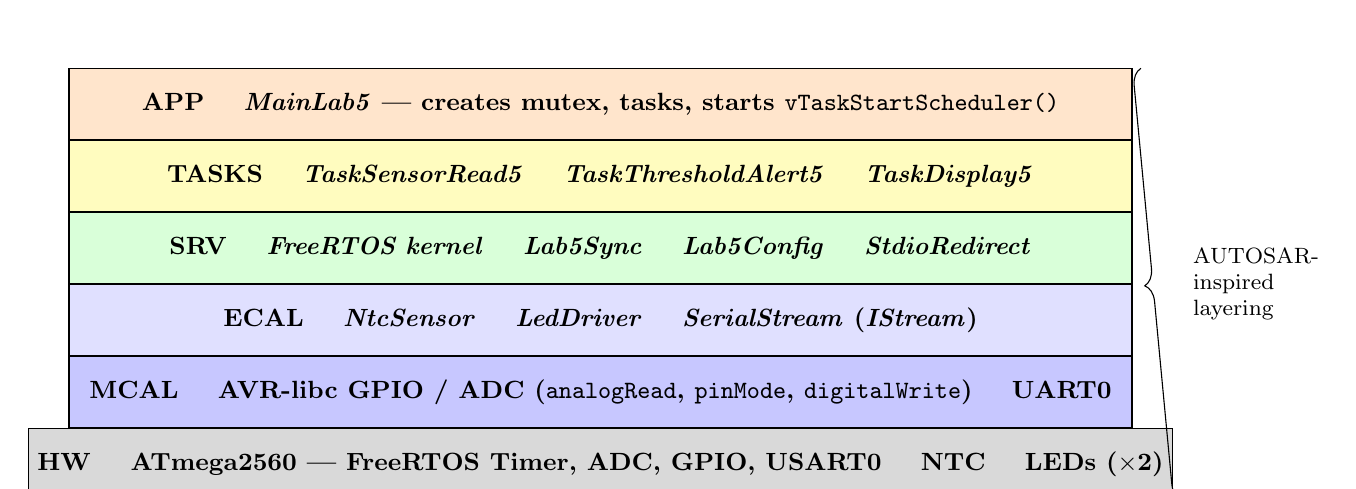
\begin{tikzpicture}[node distance=0pt]

  \def\LW{13.5cm}

  \node[layer, minimum width=\LW, fill=orange!20] (app)
    {\textbf{APP} \quad \textit{MainLab5} --- creates mutex, tasks, starts \texttt{vTaskStartScheduler()}};

  \node[layer, minimum width=\LW, fill=yellow!25, below=of app] (tasks)
    {\textbf{TASKS} \quad \textit{TaskSensorRead5} \quad \textit{TaskThresholdAlert5} \quad \textit{TaskDisplay5}};

  \node[layer, minimum width=\LW, fill=green!15, below=of tasks] (srv)
    {\textbf{SRV} \quad \textit{FreeRTOS kernel} \quad \textit{Lab5Sync} \quad \textit{Lab5Config} \quad \textit{StdioRedirect}};

  \node[layer, minimum width=\LW, fill=blue!12, below=of srv] (ecal)
    {\textbf{ECAL} \quad \textit{NtcSensor} \quad \textit{LedDriver} \quad \textit{SerialStream} (\textit{IStream})};

  \node[layer, minimum width=\LW, fill=blue!22, below=of ecal] (mcal)
    {\textbf{MCAL} \quad AVR-libc GPIO / ADC (\texttt{analogRead}, \texttt{pinMode}, \texttt{digitalWrite}) \quad UART0};

  \node[layer, minimum width=\LW, fill=gray!30, below=of mcal] (hw)
    {\textbf{HW} \quad ATmega2560 --- FreeRTOS Timer, ADC, GPIO, USART0 \quad NTC \quad LEDs ($\times$2)};

  \draw[decorate, decoration={brace, amplitude=6pt, mirror}]
    ([xshift=3pt]app.north east) -- ([xshift=3pt]hw.south east)
    node[midway, right=8pt, font=\footnotesize, align=left]
    {AUTOSAR-\\inspired\\layering};

\end{tikzpicture}
\caption{Layered Software Architecture}
\label{fig:layers}
\end{figure}

\begin{itemize}
  \item \textbf{APP}: \texttt{MainLab5} initialises hardware, creates \texttt{xLab5Mutex}, creates three FreeRTOS tasks with differentiated priorities (sensor=3, threshold=2, display=1), and starts the scheduler. \texttt{LoopLab5()} is empty --- never reached.
  \item \textbf{TASKS}: Three FreeRTOS task functions. The sensor reader has the highest priority to ensure timely ADC acquisition. The threshold alerter runs at medium priority for responsive LED control. The display task has the lowest priority since it only reports status.
  \item \textbf{SRV}: The FreeRTOS kernel provides scheduling, mutexes, and \texttt{vTaskDelayUntil}. \texttt{Lab5Sync} declares the shared volatile data and the mutex handle. \texttt{Lab5Config} holds all named constants. \texttt{StdioRedirect} connects \texttt{printf} to \texttt{SerialStream}.
  \item \textbf{ECAL}: \texttt{NtcSensor} wraps \texttt{analogRead()} and implements the Steinhart--Hart equation. \texttt{LedDriver} and \texttt{SerialStream} are reused from previous labs.
  \item \textbf{MCAL}: Arduino framework register-level abstractions, including ADC access.
  \item \textbf{HW}: Physical devices. The ATmega2560's 10-bit ADC reads the NTC voltage divider on pin A0.
\end{itemize}

\subsection{Software Module Design}

% ── Mermaid source (render externally and save as images/lab5_modules.png) ──
% ```mermaid
% classDiagram
%     class IStream {
%         <<interface>>
%         +write(char c)*
%         +read() char*
%         +available() bool*
%     }
%     class SerialStream {
%         +begin(unsigned long baud)
%         +write(char c)
%         +read() char
%         +available() bool
%     }
%     class NtcSensor {
%         +InitializeNtcSensor(uint8_t pin)
%         +ReadNtcRaw(uint8_t pin) uint16_t
%         +NtcAdcToTempC(uint16_t adc) float
%         +NtcAdcToTempC10(uint16_t adc) int16_t
%     }
%     class LedDriver {
%         +InitializeLed(int pin)
%         +SetLedState(int pin, bool on)
%     }
%     class Lab5Config {
%         +NtcAnalogPin : A0
%         +GreenLedPin5 : 12
%         +RedLedPin5 : 11
%         +ThresholdHighC : 30.0
%         +ThresholdLowC : 28.0
%         +DebounceMaxCount : 5
%         +SensorReadIntervalMs : 50
%         +ThresholdCheckMs : 50
%         +DisplayIntervalMs : 500
%     }
%     class Lab5Sync {
%         +Lab5RawAdc : volatile uint16_t
%         +Lab5TempC10 : volatile int16_t
%         +Lab5AlertActive : volatile bool
%         +Lab5RawThreshold : volatile bool
%         +Lab5DebounceCounter : volatile uint8_t
%         +xLab5Mutex : SemaphoreHandle_t
%     }
%     class TaskSensorRead5 {
%         +TaskSensorRead5Func(void*)
%     }
%     class TaskThresholdAlert5 {
%         +TaskThresholdAlert5Func(void*)
%     }
%     class TaskDisplay5 {
%         +TaskDisplay5Func(void*)
%     }
%     SerialStream ..|> IStream
%     TaskSensorRead5 --> NtcSensor : ReadNtcRaw, NtcAdcToTempC10
%     TaskSensorRead5 --> Lab5Sync : writes RawAdc, TempC10
%     TaskThresholdAlert5 --> Lab5Sync : reads TempC10, writes AlertActive
%     TaskThresholdAlert5 --> Lab5Config : thresholds, debounce
%     TaskThresholdAlert5 --> LedDriver : SetLedState
%     TaskDisplay5 --> Lab5Sync : reads all shared data
% ```

\begin{figure}[H]
\centering
\includegraphics[width=0.85\textwidth]{images/lab5_modules.png}
\caption{Software Module Diagram}
\label{fig:modules}
\end{figure}

\subsection{FreeRTOS Task Synchronisation Diagram}

% ── Mermaid source (render externally and save as images/lab5_sequence.png) ──
% ```mermaid
% sequenceDiagram
%     participant T1 as Task1: SensorRead<br/>(50ms, prio 3)
%     participant MTX as xLab5Mutex
%     participant SD as Shared Data<br/>(Lab5Sync)
%     participant T2 as Task2: ThresholdAlert<br/>(50ms, prio 2)
%     participant LED as LEDs<br/>(Green/Red)
%     participant T3 as Task3: Display<br/>(500ms, prio 1)
%
%     Note over T1: 50ms tick
%     T1->>T1: ReadNtcRaw(A0)
%     T1->>T1: NtcAdcToTempC10(raw)
%     T1->>MTX: xSemaphoreTake()
%     T1->>SD: Lab5RawAdc = raw
%     T1->>SD: Lab5TempC10 = tempC10
%     T1->>MTX: xSemaphoreGive()
%
%     Note over T2: 50ms tick
%     T2->>MTX: xSemaphoreTake()
%     T2->>SD: read Lab5TempC10
%     T2->>MTX: xSemaphoreGive()
%     T2->>T2: hysteresis comparison
%     T2->>T2: debounce counter update
%     T2->>LED: SetLedState(green/red)
%     T2->>MTX: xSemaphoreTake()
%     T2->>SD: write AlertActive, RawThreshold, DebounceCounter
%     T2->>MTX: xSemaphoreGive()
%
%     Note over T3: 500ms tick
%     T3->>MTX: xSemaphoreTake()
%     T3->>SD: snapshot all fields
%     T3->>MTX: xSemaphoreGive()
%     T3->>T3: printf_P() status line
% ```

\begin{figure}[H]
\centering
\includegraphics[width=0.85\textwidth]{images/lab5_sequence.png}
\caption{FreeRTOS Task Synchronisation Sequence}
\label{fig:sequence}
\end{figure}

The synchronisation architecture:
\begin{itemize}
  \item \textbf{xLab5Mutex}: A single mutex protects all five shared volatile variables. Each task acquires the mutex only for the minimum duration needed to read or write the shared data, minimising contention.
  \item \textbf{Priority assignment}: Task~1 (sensor read) has the highest priority (3) to ensure timely ADC acquisition. Task~2 (threshold alert) at priority~2 ensures responsive LED control. Task~3 (display) at priority~1 yields to sensor and alert processing.
  \item \textbf{No semaphore needed}: Unlike Lab~1.4, there is no producer-consumer event signalling. All three tasks run periodically, and the threshold alert reads the latest available temperature value.
\end{itemize}

\subsection{Threshold Alerting --- State Machine with Hysteresis}

\begin{figure}[H]
\centering
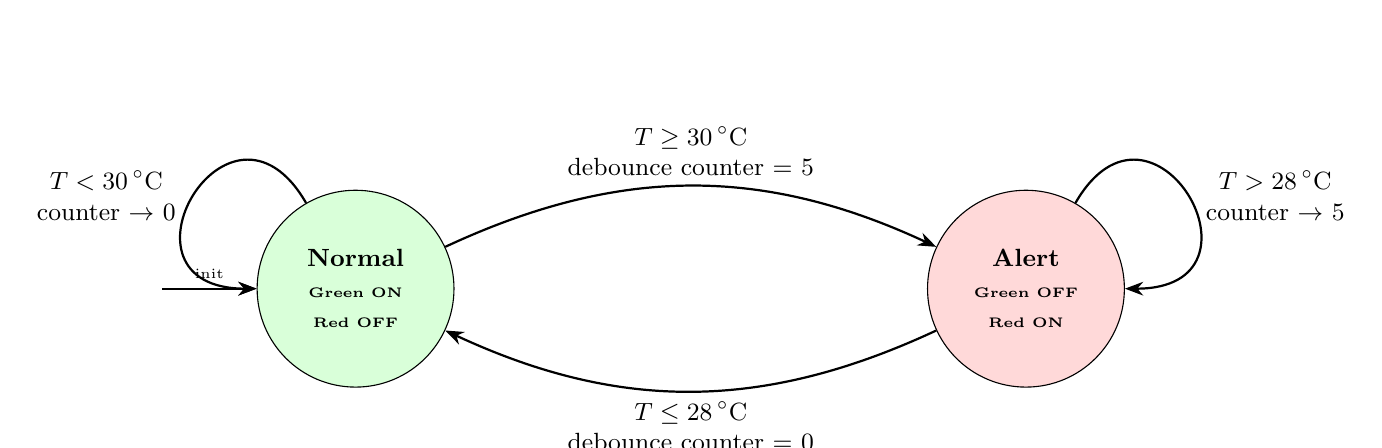
\begin{tikzpicture}[
  state/.style={circle, draw, fill=blue!10, minimum size=2.5cm,
                align=center, font=\small\bfseries},
  arr/.style={-Stealth, thick},
  node distance=6.0cm
]
  \node[state, fill=green!15] (normal) {Normal\\{\tiny Green ON}\\{\tiny Red OFF}};
  \node[state, fill=red!15, right=of normal] (alert) {Alert\\{\tiny Green OFF}\\{\tiny Red ON}};

  \draw[arr, bend left=25] (normal) to
    node[above, font=\small, align=center]
      {$T \geq 30\,^{\circ}$C\\debounce counter = 5}
    (alert);

  \draw[arr, bend left=25] (alert) to
    node[below, font=\small, align=center]
      {$T \leq 28\,^{\circ}$C\\debounce counter = 0}
    (normal);

  \draw[arr] (normal.120) to[out=120, in=180, looseness=4]
    node[left, font=\small, xshift=-3pt, align=center]{$T < 30\,^{\circ}$C\\counter $\to$ 0}
    (normal.180);

  \draw[arr] (alert.60) to[out=60, in=0, looseness=4]
    node[right, font=\small, xshift=3pt, align=center]{$T > 28\,^{\circ}$C\\counter $\to$ 5}
    (alert.0);

  \draw[arr] ($(normal.west)+(-1.2,0)$) -- (normal.west)
    node[midway, above, font=\tiny]{init};

\end{tikzpicture}
\caption{Threshold Alert --- Finite State Machine with Hysteresis and Debounce}
\label{fig:fsm}
\end{figure}

The hysteresis band of 2\,\(^{\circ}\)C (\(T_{high} = 30\,^{\circ}\)C, \(T_{low} = 28\,^{\circ}\)C) combined with a debounce counter of 5 samples provides robust binary classification. The debounce window is \(5 \times 50\text{\,ms} = 250\text{\,ms}\), which filters transient temperature spikes while maintaining acceptable response time.

\subsection{Electronic Design}

\begin{figure}[H]
\centering
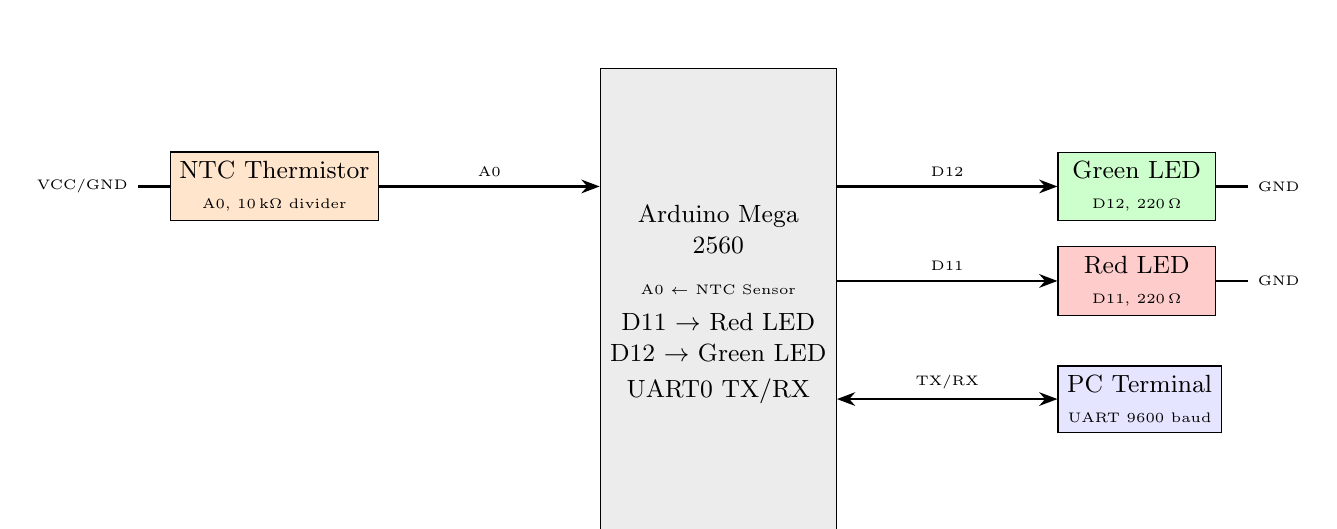
\begin{tikzpicture}[
  blk/.style={rectangle, draw, minimum height=1.4cm, align=center, font=\small},
  mcu/.style={blk, fill=gray!15, minimum width=3.0cm, minimum height=6.0cm},
  ledb/.style={blk, fill=green!20, minimum width=2.0cm, minimum height=0.75cm},
  ledr/.style={blk, fill=red!20,   minimum width=2.0cm, minimum height=0.75cm},
  snsb/.style={blk, fill=orange!20, minimum width=2.0cm, minimum height=0.75cm},
  bus/.style={-Stealth, thick},
  lbl/.style={font=\tiny, midway},
]

  \node[mcu] (mcu) {Arduino Mega\\2560\\[4pt]
    \tiny A0 $\leftarrow$ NTC Sensor\\[2pt]
    D11 $\to$ Red LED\\D12 $\to$ Green LED\\[2pt]
    UART0 TX/RX};

  \node[snsb, left=2.8cm of mcu, yshift=1.5cm] (ntc)
    {NTC Thermistor\\{\tiny A0, 10\,k$\Omega$ divider}};

  \node[ledb, right=2.8cm of mcu, yshift=1.5cm] (gled)
    {Green LED\\{\tiny D12, 220\,$\Omega$}};

  \node[ledr, right=2.8cm of mcu, yshift=0.3cm] (rled)
    {Red LED\\{\tiny D11, 220\,$\Omega$}};

  \node[blk, fill=blue!10, minimum width=2.0cm, minimum height=0.75cm, right=2.8cm of mcu, yshift=-1.2cm] (ser)
    {PC Terminal\\{\tiny UART 9600 baud}};

  \draw[bus] (ntc.east) -- node[lbl, above]{A0} (mcu.west |- ntc.east);

  \draw[bus] (mcu.east |- gled.west) -- node[lbl, above]{D12} (gled.west);
  \draw[bus] (mcu.east |- rled.west) -- node[lbl, above]{D11} (rled.west);
  \draw[bus, Stealth-Stealth] (mcu.east |- ser.west) --
    node[lbl, above]{TX/RX} (ser.west);

  \foreach \led in {gled, rled}
    \draw[thick] (\led.east) -- ++(0.4,0) node[right, font=\tiny]{GND};

  \draw[thick] (ntc.west) -- ++(-0.4,0) node[left, font=\tiny]{VCC/GND};

\end{tikzpicture}
\caption{Electronic Design --- Pin Connection Diagram}
\label{fig:elec}
\end{figure}

\begin{itemize}
  \item \textbf{NTC Thermistor (A0)}: Connected in a voltage divider. VCC $\to$ $R_{fixed}$ (10\,k$\Omega$) $\to$ A0 $\to$ NTC $\to$ GND. The ADC reads the midpoint voltage.
  \item \textbf{Green LED (D12)}: Normal state indicator. 220\,$\Omega$ series resistor. ON when temperature is below the alert threshold.
  \item \textbf{Red LED (D11)}: Alert state indicator. Same resistor topology. ON when temperature exceeds the threshold (after debounce).
  \item \textbf{UART0 (TX/RX)}: 9600\,baud serial connection for the 500\,ms status display.
\end{itemize}

% ─────────────────────────────────────────────────────────────────────────────
\section{Implementation}
% ─────────────────────────────────────────────────────────────────────────────

\subsection{Project Structure}

\begin{table}[H]
\centering
\begin{tabular}{@{}lp{8.2cm}@{}}
\toprule
\textbf{File} & \textbf{Purpose} \\
\midrule
\texttt{src/main.cpp}
  & Lab selector; dispatches \texttt{setup()}/\texttt{loop()} based on \texttt{ACTIVE\_LAB} \\
\texttt{src/labs/lab5/MainLab5.cpp}
  & Creates mutex and three FreeRTOS tasks; calls \texttt{vTaskStartScheduler()} \\
\texttt{src/labs/lab5/TaskSensorRead5.cpp}
  & 50\,ms periodic ADC read with Steinhart--Hart conversion \\
\texttt{src/labs/lab5/TaskThresholdAlert5.cpp}
  & 50\,ms periodic hysteresis threshold check with debounce \\
\texttt{src/labs/lab5/TaskDisplay5.cpp}
  & 500\,ms periodic status display via \texttt{printf\_P} \\
\texttt{src/components/NtcSensor.cpp}
  & ADC read, Steinhart--Hart conversion, linear mapping \\
\texttt{src/components/LedDriver.cpp}
  & \texttt{InitializeLed} / \texttt{SetLedState} --- GPIO output \\
\texttt{src/components/SerialStream.cpp}
  & \texttt{IStream} implementation over \texttt{HardwareSerial} \\
\texttt{src/components/StdioRedirect.cpp}
  & \texttt{initStdio(IStream*)} via \texttt{fdev\_setup\_stream} \\
\texttt{include/labs/lab5/Lab5Config.h}
  & Named constants: pins, thresholds, debounce count, task timing \\
\texttt{include/labs/lab5/Lab5Sync.h}
  & Declares shared \texttt{volatile} data and \texttt{xLab5Mutex} \\
\texttt{include/drivers/NtcSensor.h}
  & NTC parameters (\(R_0\), \(T_0\), \(B\), \(R_{fixed}\)); function declarations \\
\bottomrule
\end{tabular}
\caption{Project File Structure}
\label{tab:files}
\end{table}

\subsection{PlatformIO Environment Configuration}

The build is selected via the \texttt{[env:mega\_lab5]} environment in \texttt{platformio.ini}:

\begin{lstlisting}
[env:mega_lab5]
extends = env:mega
build_flags =
    -D USE_FREERTOS
    -D ACTIVE_LAB=5
\end{lstlisting}

This environment extends \texttt{env:mega}, inheriting the ATmega2560 board, Arduino framework, and \texttt{feilipu/FreeRTOS@\^{}10.5.1-1} dependency. The \texttt{-D USE\_FREERTOS} flag guards bare-metal ISR code to avoid conflicts with the FreeRTOS tick timer.

\subsection{Configuration Constants}

All configuration values are defined as named constants in \texttt{Lab5Config.h}:

\begin{lstlisting}[caption={Lab5Config.h --- configuration constants}]
const uint8_t NtcAnalogPin  = A0;
const uint8_t GreenLedPin5  = 12;   // normal state
const uint8_t RedLedPin5    = 11;   // alert state

const float ThresholdHighC  = 30.0f;   // upper threshold
const float ThresholdLowC   = 28.0f;   // lower threshold
const uint8_t DebounceMaxCount = 5;

const uint16_t SensorReadIntervalMs   = 50;
const uint16_t ThresholdCheckMs       = 50;
const uint16_t DisplayIntervalMs      = 500;
\end{lstlisting}

\subsection{Shared Data and Synchronisation}

The shared state is declared in \texttt{Lab5Sync.h}, conditionally compiled under \texttt{USE\_FREERTOS}:

\begin{lstlisting}[caption={Lab5Sync.h --- shared volatile data and mutex}]
#pragma once
#ifdef USE_FREERTOS
#include <Arduino_FreeRTOS.h>
#include <semphr.h>

extern volatile uint16_t Lab5RawAdc;
extern volatile int16_t  Lab5TempC10;
extern volatile bool     Lab5AlertActive;
extern volatile bool     Lab5RawThreshold;
extern volatile uint8_t  Lab5DebounceCounter;

extern SemaphoreHandle_t xLab5Mutex;
#endif
\end{lstlisting}

All five shared variables are declared \texttt{volatile} to prevent compiler optimisations that could cause stale reads across task contexts.

\subsection{Task Setup and Scheduler Launch}

\texttt{SetupLab5()} in \texttt{MainLab5.cpp} performs the following steps:
\begin{enumerate}
  \item Initialise serial at 9600\,baud and hook STDIO via \texttt{initStdio(\&SerialIo)}.
  \item Initialise the NTC sensor pin (A0) and two LEDs (D11, D12).
  \item Set initial LED states: green ON, red OFF.
  \item Create the mutex: \texttt{xLab5Mutex = xSemaphoreCreateMutex()}.
  \item Create three tasks with differentiated priorities: Sensor (128 words, prio~3), Threshold (128 words, prio~2), Display (256 words, prio~1).
  \item Print a welcome message via \texttt{printf\_P}.
  \item Call \texttt{vTaskStartScheduler()} --- does not return.
\end{enumerate}

\begin{lstlisting}[caption={SetupLab5 --- task creation and scheduler launch}]
void SetupLab5() {
    SerialIo.begin(9600);
    initStdio(&SerialIo);

    InitializeNtcSensor(NtcAnalogPin);
    InitializeLed(GreenLedPin5);
    InitializeLed(RedLedPin5);

    SetLedState(GreenLedPin5, true);
    SetLedState(RedLedPin5, false);

    xLab5Mutex = xSemaphoreCreateMutex();

    xTaskCreate(TaskSensorRead5Func,    "Sensor",
                128, nullptr, 3, nullptr);
    xTaskCreate(TaskThresholdAlert5Func,"Threshold",
                128, nullptr, 2, nullptr);
    xTaskCreate(TaskDisplay5Func,       "Display",
                256, nullptr, 1, nullptr);

    printf_P(PSTR("Lab 5: Binary Signal - Threshold "
                  "Alerting\n"));
    printf_P(PSTR("Sensor: NTC on A0\n"));
    printf_P(PSTR("Alert: >%d C (hyst: %d C)\n"),
        (int)ThresholdHighC, (int)ThresholdLowC);
    printf_P(PSTR("Green=normal, Red=alert\n"));

    vTaskStartScheduler();
}
\end{lstlisting}

\subsection{NTC Sensor Driver}

The \texttt{NtcSensor} module provides the ADC reading and Steinhart--Hart conversion:

\begin{lstlisting}[caption={NtcSensor --- ADC read and temperature conversion}]
uint16_t ReadNtcRaw(uint8_t analogPin) {
    return (uint16_t)analogRead(analogPin);
}

float NtcAdcToTempC(uint16_t adcValue) {
    if (adcValue == 0) adcValue = 1;
    if (adcValue >= 1023) adcValue = 1022;

    float resistance = NtcRFixed * (float)adcValue
                     / (1023.0f - (float)adcValue);

    float steinhart = log(resistance / NtcR0) / NtcBeta;
    steinhart += 1.0f / NtcT0K;
    float temperatureK = 1.0f / steinhart;

    return temperatureK - 273.15f;
}

int16_t NtcAdcToTempC10(uint16_t adcValue) {
    float tempC = NtcAdcToTempC(adcValue);
    return (int16_t)(tempC * 10.0f);
}
\end{lstlisting}

The ADC value is clamped to [1, 1022] to prevent division by zero. The resistance is computed from the voltage divider equation, then the Steinhart--Hart Beta equation converts resistance to temperature. \texttt{NtcAdcToTempC10()} returns temperature in tenths of a degree for integer display formatting.

\subsection{TaskSensorRead5Func --- Sensor Acquisition}

The sensor task reads the ADC every 50\,ms, converts to temperature, and writes both values to shared memory under mutex protection:

\begin{lstlisting}[caption={TaskSensorRead5Func --- periodic sensor acquisition}]
void TaskSensorRead5Func(void* pvParameters) {
    const TickType_t Interval =
        pdMS_TO_TICKS(SensorReadIntervalMs);
    TickType_t xLastWakeTime = xTaskGetTickCount();

    for (;;) {
        uint16_t raw = ReadNtcRaw(NtcAnalogPin);
        int16_t tempC10 = NtcAdcToTempC10(raw);

        xSemaphoreTake(xLab5Mutex, portMAX_DELAY);
        Lab5RawAdc  = raw;
        Lab5TempC10 = tempC10;
        xSemaphoreGive(xLab5Mutex);

        vTaskDelayUntil(&xLastWakeTime, Interval);
    }
}
\end{lstlisting}

The ADC read and Steinhart--Hart conversion are performed \emph{outside} the mutex to minimise the critical section duration. Only the two shared variable writes are protected.

\subsection{TaskThresholdAlert5Func --- Hysteresis and Debounce}

The threshold alert task implements the hysteresis state machine with debounce counter:

\begin{lstlisting}[caption={TaskThresholdAlert5Func --- hysteresis + debounce}]
void TaskThresholdAlert5Func(void* pvParameters) {
    const TickType_t Interval =
        pdMS_TO_TICKS(ThresholdCheckMs);
    TickType_t xLastWakeTime = xTaskGetTickCount();

    const int16_t ThreshHighC10 =
        (int16_t)(ThresholdHighC * 10.0f);
    const int16_t ThreshLowC10  =
        (int16_t)(ThresholdLowC * 10.0f);

    bool alertState = false;
    uint8_t counter = 0;

    for (;;) {
        xSemaphoreTake(xLab5Mutex, portMAX_DELAY);
        int16_t tempC10 = Lab5TempC10;
        xSemaphoreGive(xLab5Mutex);

        bool rawState;
        if (!alertState) {
            rawState = (tempC10 >= ThreshHighC10);
        } else {
            rawState = (tempC10 > ThreshLowC10);
        }

        if (rawState) {
            if (counter < DebounceMaxCount) counter++;
        } else {
            if (counter > 0) counter--;
        }

        if (counter >= DebounceMaxCount) {
            alertState = true;
        } else if (counter == 0) {
            alertState = false;
        }

        SetLedState(GreenLedPin5, !alertState);
        SetLedState(RedLedPin5,    alertState);

        xSemaphoreTake(xLab5Mutex, portMAX_DELAY);
        Lab5AlertActive     = alertState;
        Lab5RawThreshold    = rawState;
        Lab5DebounceCounter = counter;
        xSemaphoreGive(xLab5Mutex);

        vTaskDelayUntil(&xLastWakeTime, Interval);
    }
}
\end{lstlisting}

Key implementation details:
\begin{itemize}
  \item The threshold comparison depends on the current \texttt{alertState}: in the normal state, the temperature must reach \(T_{high}\) to trigger; in the alert state, it must drop below \(T_{low}\) to clear. This is the hysteresis mechanism.
  \item The debounce counter increments or decrements toward the target, requiring 5 consecutive confirmations (250\,ms) before committing the state change.
  \item LED updates occur \emph{before} writing to shared data, ensuring the physical output reflects the decision immediately.
  \item The mutex is acquired twice: once for reading the temperature (input), once for writing the alert state (output). This minimises lock duration.
\end{itemize}

\subsection{TaskDisplay5Func --- Status Display}

The display task snapshots all shared data under mutex and emits a formatted status line every 500\,ms:

\begin{lstlisting}[caption={TaskDisplay5Func --- periodic status display}]
void TaskDisplay5Func(void* pvParameters) {
    const TickType_t Interval =
        pdMS_TO_TICKS(DisplayIntervalMs);
    TickType_t xLastWakeTime = xTaskGetTickCount();

    for (;;) {
        vTaskDelayUntil(&xLastWakeTime, Interval);

        xSemaphoreTake(xLab5Mutex, portMAX_DELAY);
        uint16_t raw       = Lab5RawAdc;
        int16_t  tempC10   = Lab5TempC10;
        bool     alert     = Lab5AlertActive;
        bool     rawThresh = Lab5RawThreshold;
        uint8_t  debounce  = Lab5DebounceCounter;
        xSemaphoreGive(xLab5Mutex);

        int16_t whole = tempC10 / 10;
        uint16_t frac = (uint16_t)(tempC10 < 0
            ? -(tempC10 % 10) : (tempC10 % 10));

        printf_P(PSTR("RAW:%u T:%d.%uC Thr:%c "
            "Deb:%u/%u Alert:%s\n"),
            raw, whole, frac,
            rawThresh ? 'H' : 'L',
            debounce, DebounceMaxCount,
            alert ? "ON" : "OFF");
    }
}
\end{lstlisting}

The output includes: raw ADC value, temperature with one decimal place, raw threshold state (H/L), debounce counter progress, and the debounced alert status (ON/OFF). The \texttt{vTaskDelayUntil} is placed at the \emph{beginning} of the loop to allow time for sensor initialisation before the first display.

\subsection{STDIO Usage}

\begin{table}[H]
\centering
\begin{tabular}{@{}lp{4cm}p{5.5cm}@{}}
\toprule
\textbf{Function} & \textbf{Call site} & \textbf{Output} \\
\midrule
\texttt{printf\_P}
  & \texttt{SetupLab5} (4$\times$)
  & Welcome message, sensor info, threshold values \\
\texttt{printf\_P}
  & \texttt{TaskDisplay5Func}
  & 500\,ms status: RAW, temperature, threshold, debounce, alert \\
\bottomrule
\end{tabular}
\caption{STDIO Usage}
\label{tab:stdio}
\end{table}

\subsection{Code}

The full source code is available at the GitHub repository listed as the first entry in the bibliography \cite{code}.

% ─────────────────────────────────────────────────────────────────────────────
\section{Results}
% ─────────────────────────────────────────────────────────────────────────────

The application was verified in simulation and on hardware. The following scenarios were tested:

\begin{enumerate}
  \item \textbf{Welcome message}: On power-up, four lines are printed: ``Lab 5: Binary Signal - Threshold Alerting'', sensor type, alert thresholds, and LED assignments.

  \item \textbf{Normal state}: When the temperature is below 28\,\(^{\circ}\)C, the green LED is ON, the red LED is OFF, and the display shows ``Alert:OFF''.

  \item \textbf{Rising above threshold}: When the temperature rises above 30\,\(^{\circ}\)C, the raw threshold changes to H and the debounce counter increments. After 5 consecutive samples (250\,ms), the alert activates: red LED ON, green LED OFF, display shows ``Alert:ON''.

  \item \textbf{Falling below threshold}: When the temperature drops below 28\,\(^{\circ}\)C, the raw threshold changes to L and the counter decrements. After reaching 0, the alert deactivates.

  \item \textbf{Hysteresis dead band}: Temperatures between 28\,\(^{\circ}\)C and 30\,\(^{\circ}\)C do not cause state transitions --- the system maintains its current state.

  \item \textbf{Debounce filtering}: Brief temperature spikes above 30\,\(^{\circ}\)C (lasting fewer than 5 samples) do not trigger the alert.
\end{enumerate}

A sample serial monitor output:

\begin{lstlisting}
Lab 5: Binary Signal - Threshold Alerting
Sensor: NTC on A0
Alert: >30 C (hyst: 28 C)
Green=normal, Red=alert
RAW:512 T:25.3C Thr:L Deb:0/5 Alert:OFF
RAW:510 T:25.4C Thr:L Deb:0/5 Alert:OFF
RAW:480 T:28.1C Thr:L Deb:0/5 Alert:OFF
RAW:450 T:31.2C Thr:H Deb:1/5 Alert:OFF
RAW:448 T:31.5C Thr:H Deb:2/5 Alert:OFF
RAW:445 T:31.8C Thr:H Deb:5/5 Alert:ON
RAW:460 T:30.5C Thr:H Deb:5/5 Alert:ON
RAW:490 T:27.8C Thr:L Deb:4/5 Alert:ON
RAW:492 T:27.5C Thr:L Deb:0/5 Alert:OFF
\end{lstlisting}

\subsection{Test Validation}

\begin{table}[H]
\centering
\begin{tabular}{@{}llp{7.5cm}@{}}
\toprule
\textbf{Test ID} & \textbf{Result} & \textbf{Observations} \\
\midrule
RF01\_T01  & Pass & ADC reads NTC value correctly every 50\,ms. \\
RF02\_T01  & Pass & Steinhart--Hart conversion produces accurate temperature. \\
RF03\_T01  & Pass & Hysteresis prevents toggling in the 28--30\,\(^{\circ}\)C dead band. \\
RF04\_T01  & Pass & Debounce counter requires 5 consecutive samples to confirm. \\
RF05\_T01  & Pass & Green LED indicates normal; red LED indicates alert. \\
RF06\_T01  & Pass & Display task shows all pipeline values every 500\,ms. \\
RNF01\_T01 & Pass & Tasks run concurrently; no shared data corruption observed. \\
RNF02\_T01 & Pass & Code is modular with separate files per component. \\
RNF03\_T01 & Pass & Mutex protects all shared volatile variables. \\
RNF04\_T01 & Pass & All configuration values are named constants. \\
RNF05\_T01 & Pass & Sensor latency under 50\,ms (single task period). \\
RNF06\_T01 & Pass & PROGMEM strings conserve SRAM on ATmega2560. \\
\bottomrule
\end{tabular}
\caption{Test Results for the Threshold Alerting Application}
\label{tab:tests}
\end{table}

% ─────────────────────────────────────────────────────────────────────────────
\section{Note on AI}
% ─────────────────────────────────────────────────────────────────────────────

\hspace{0.8cm}
For this laboratory work, AI assistants such as Claude~4.6~Sonnet were used for explaining code sections, underlying technologies (Steinhart--Hart equation, hysteresis threshold design, FreeRTOS task priorities), and for assisting with debugging. They were also used for paraphrasing and structuring ideas in this report. All AI-generated content was reviewed and verified against the actual implementation.

% ─────────────────────────────────────────────────────────────────────────────
\section{Conclusion}
% ─────────────────────────────────────────────────────────────────────────────

\hspace{0.8cm}
This laboratory work demonstrated binary signal monitoring using an NTC thermistor with FreeRTOS on an ATmega2560. The application reads the analog sensor, converts the ADC value to temperature via the Steinhart--Hart equation, and applies threshold alerting with hysteresis and debouncing to produce a robust binary classification (normal/alert).

\hspace{0.8cm}
The hysteresis band of 2\,\(^{\circ}\)C prevents rapid toggling near the threshold, and the debounce counter (5~samples, 250\,ms window) filters transient temperature spikes. Together, these mechanisms ensure that the alert state changes only in response to sustained temperature shifts, not noise.

\hspace{0.8cm}
The three FreeRTOS tasks are prioritised by function: the sensor reader has the highest priority to ensure timely acquisition, the threshold alerter runs at medium priority for responsive LED control, and the display task has the lowest priority. A single mutex protects all shared volatile data with minimal critical section duration. This architecture builds on the FreeRTOS infrastructure from Lab~1.4 and provides the foundation for the signal conditioning pipeline in Lab~1.6.

% ─────────────────────────────────────────────────────────────────────────────
\section{Bibliography}
% ─────────────────────────────────────────────────────────────────────────────

\begingroup
\makeatletter
\renewcommand{\section}[2]{}
\makeatother

\begin{thebibliography}{}

  \bibitem{code}
  \url{https://github.com/NeValetik/si-labs}

  \bibitem{ntc_steinhart}
  Ametherm. \textit{NTC Thermistors --- Steinhart and Hart Equation}.
  \url{https://www.ametherm.com/thermistor/ntc-thermistor-steinhart-hart-equation}

  \bibitem{freertos_mutex}
  FreeRTOS. \textit{Mutexes}.
  \url{https://www.freertos.org/Documentation/02-Kernel/02-Kernel-features/02-Queues-mutexes-and-semaphores/04-Mutexes}

  \bibitem{freertos_tasks}
  FreeRTOS. \textit{Task Creation}.
  \url{https://www.freertos.org/Documentation/02-Kernel/04-API-references/01-Task-creation/00-TaskCreate}

  \bibitem{pio}
  PlatformIO. \textit{PlatformIO Documentation --- atmelavr Platform}.
  \url{https://docs.platformio.org/en/latest/platforms/atmelavr.html}

  \bibitem{avr}
  Microchip Technology. \textit{ATmega2560 Datasheet}, DS40002211A, 2020.
  \url{https://ww1.microchip.com/downloads/en/devicedoc/atmel-2549-8-bit-avr-microcontroller-atmega640-1280-1281-2560-2561_datasheet.pdf}

\end{thebibliography}
\endgroup

\pagebreak
\end{document}
